\documentclass[10pt,final,a4paper,oneside]{article}
%\documentclass[10pt,journal,final,a4paper,twoside]{IEEEtran}
%\documentclass[10pt,journal,draftclsnofoot,a4paper]{IEEEtran}
%\documentclass[10pt,journal,draftclsnofoot,onecolumn,a4paper]{IEEEtran}
%\documentclass[10pt,journal,final,onecolumn,a4paper]{IEEEtran}

\usepackage{cite}
\usepackage{graphicx}

\begin{document}
\title{Web Services with eZ Components:\\ A Design Proposal}
\author{Falko~Menge and Stefan~Marr}
\markboth{Web Services with eZ Components}{Falko Menge and Stefan Marr}

\maketitle


\begin{abstract}
This paper describes the current design state
of the InstantSVC core libraries.
It serves as a foundation for discussing the contribution
of these core libraries to the eZ Components project.
Therefore it proposes six new components:
ezcReflection, ezcCodeAnalyzer, ezcWsdl, ezcSoap, ezcRest and ezcWebService.
For each component requirements and design are specified.
\end{abstract}

\section{Web Services and PHP5}\label{sec:Introduction}
Web services are one of the most interesting technologies to evolve in the
last years. They facilitate interoperable communication across the borders of 
platforms and programming languages and are therefore a very 
promising concept for enterprise software. They can be used to integrate 
internal software systems as well as cross-company applications. The main idea is that 
applications provide their functionality in form of services that can be 
used by other applications via network or even internet. 

The standards that form the foundation for Web Services are the SOAP
protocol \cite{SOAP}, the Web Services Description Language (WSDL) \cite{WSDL},
Universal Description, Discovery and Integration (UDDI) \cite{UDDI} and the
Hypertext Transfer Protocol (HTTP) \cite{HTTP}.
SOAP is the messaging protocol used to access the services. WSDL is an
open standard for XML-based service interface descriptions which serve as
contracts between service providers and consumers. Name services for
publishing and searching Web Services are specified by UDDI. HTTP is
leveraged as transport protocol for SOAP messages and in case of ReSTful
Web Services it even serves as a universal and minimal interface to all
services.

For efficient utilization of SOAP and in most cases also WSDL
sophisticated tools have been developed for all major programming
languages and platforms.
Since UDDI is itself a Web Service there is no need
to reimplement it for every platform or language.
Instead several Open Source or commercial products are available.
PHP5 also incorporates a SOAP implementation with support for WSDL
in form of an extension module.

In order to expose a PHP class as a Web Service using this SOAP extension
several steps have to be performed.
At first an interface description has to be created using WSDL. This includes
defining XML Schema expressions \cite{XMLSchema} which specify for all data types
used by methods of the class how they should be represented inside SOAP messages.
The methods themselves become WSDL operations which use the XML Schema types.
If documentation should be provided together with the WSDL description,
the developer may copy the source code documentation into
WSDL documentation elements.
The last step would be to program a PHP application which starts a SOAP server
using the WSDL file, then passes the class name to this server and tells it to
handle SOAP requests arriving via HTTP POST.

Of course performing this procedure manually is not what was meant by
convenient tool support.
The SOAP extension is easy to use. However especially writing WSDL by hand is not
acceptable for professional developers who want to build service-oriented
architectures with maybe hundreds of services. Other platforms like e.g.
Java EE or .NET typically use annotation mechanisms to tag classes and methods
for publication as Web Services. The tagged source code is then processed by a
sophisticated tool chain which generates WSDL descriptions, additional source code
for stubs and skeletons and if needed deployment descriptors for the desired
runtime environment.
After that the services are ready for instant deployment.
Of course PHP needs no stubs because the SOAP client can use the dynamic
features of the language to create response objects at runtime.
However the same dynamic features make it difficult to generate WSDL from PHP
code because there is no type information in it.
The aim of our work was to eliminate the lack of tool support for PHP.

The paper is divided into six main sections
with each of them describing one proposal
for a new component of the tool chain.
The descriptions will focus especially on architecture and design decisions.
Following the development process of eZ Components each section consists of two parts.
A first part describes the requirements for a component and while the other one
specifies a design.



\section{Reflection}\label{sec:Reflection}
%eZ component: Reflection, Requirements
%~~~~~~~~~~~~~~~~~~~~~~~~~~~~~~~~~
%
\subsection{Introduction}
%============
Since Web Services have been invented
to enable interoperable communication between
various platforms they have to be statically typed.
Hence type information will be required when
developing tools for automated generation of Web Services.
In modern programming languages
a typical way to obtain structural information
is to leverage the runtime environment of the language
and access language elements through a high level reflection API.

As of PHP5 a Reflection API has been included
in the standard PHP distribution.
It provides an API to obtain information about classes
and all their methods and properties,
without the need to parse any source code.
Simple functions, runtime objects and PHP extensions
can be inspected, as well.
But information gathering is not the
only feature of the Reflection API.
It is also possible to modify properties of objects,
invoke arbitrary methods or functions and
instantiate objects.

\begin{figure}[htbp]
	\centering
		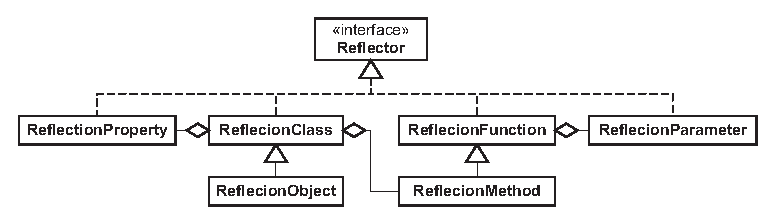
\includegraphics[width=1.00\textwidth]{figures/php5-reflection-api.eps}
	\caption{Class diagram of the  PHP5 Reflection API}
	\label{fig:php5-reflection-api}
\end{figure}

As shown in Figure \ref{fig:php5-reflection-api}
the Reflection API conforms to a meta model
of an object-oriented programming language.
That way it is possible to reflect
nearly all aspects of a given class or object.

However PHP's Reflection API does not provide any type information
due to PHP being a dynamically typed language.
That means only types of concrete variables or objects
at runtime can be determined.
But it is not possible to obtain this information statically from
class or function declarations without having an instance.
This is indeed not a problem for implementing SOAP
since it only deals with concrete instances at runtime.
But e.g. when describing service interfaces
the knowledge of structural details is essentially required.

When looking at professional PHP applications
it stands out that they only use the dynamic
typing features where they really make sense.
Large parts of the code will work with strict
types and even enforce them e.g. by throwing
an exception when receiving input of a wrong data type.
This behavior is also documented in the source code
documentation stored in comments of those language elements.
Thus it appears that in many cases type information
already exists statically in the source code.

With version 5.1 of PHP the capabilities of the Reflection API
have been enhanced and now it is possible to extract all comments
associated to a language construct with API methods.
So it is a logical next step to leverage the information
given in the source code documentation directly at runtime.

phpDocumentor \cite{phpDocumentor} the standard documentation tool for PHP
provides a common way to document source code and
uses a formal syntax which can be processed by a computer.
Unfortunately just the syntax for data type descriptions
is somewhat underspecified since it was only meant
to be understandable by human beings.
In order to parse these data type descriptions
the syntax has to be specified more precisely
as defined in section \ref{subsubsec:ReflectionFormat}.

Given a technology to access documentation tags
at runtime it would be a perfect foundation
to build an annotation mechanism for PHP
since it would be also feasible to introduce and work with new tags.
Interestingly there have been comparable developments in other
programming languages e.g. in Java with XDoclet.


\subsubsection{Description}
%-----------
The main objective of the Reflection component is
to enhance PHP by type information and annotations.
It uses source code documentation to determine
data types and other pieces of information provided
via annotations.
Those annotations can be used to realize systems
which depend on strong type information or
additional details about the source code itself.


\subsubsection{Current implementation}
%----------------------
The current implementation is highly evolved and well tested.
The component is already used by several tools
and can be considered stable.


\subsection{Requirements}\label{subsec:ReflectionRequirements}
%Requirements
%============
The Reflection component should have
the same features, power and performance
as the original Reflection API
but enhanced by the ability to obtain annotations
for classes, methods, properties or functions.
This new feature should also be used
to implement a type system
which enables PHP applications to retrieve
data types of parameters, return values and properties.

The type system should distinguish between three main categories of types.
Primitive Types are the build in types boolean, integer, double, string and resource.
Array Types are all kinds of arrays and
Class Types are used to represent user defined or internal classes.
This differentiation is made
in consideration of the language behavior
and the capabilities of WSDL for defining types
in a language independent way.
Since arrays are treated in a special way
they are additionally classified as simple arrays or maps.
An array is represented as a map if it is an associative array
i.e. is used like key value pairs.

Usage scenarios of the Reflection component are
e.g. WSDL generation for Web Services
or Aspect-Oriented Programming (AOP).
Processable additions to the source code in general
enable a wide range of new applications.

\subsubsection{Design goals}
%============
The Reflection API of PHP should be extended
as much as possible through class inheritance.

\subsubsection{Special considerations}
%======================
In order to maintain the dynamic nature of the language
it is explicitly not required
to enforce any constraints at runtime.
The PHP language runtime should not be modified at all.
As a consequence the component expects a correct source code documentation
and it is possible that runtime behavior does not correspond
to the behavior expected due to improper documentation.

\subsubsection{Format}\label{subsubsec:ReflectionFormat}
%======
The Reflection component should reuse the syntax
of phpDocumentor \cite{phpDocumentor}
and also some of its annotation tags.
To retrieve the data types of properties,
parameters and return values the annotations
\verb|@var|,
\verb|@param| and
\verb|@return| should be analyzed.
They have the following syntax:

\begin{verbatim}
/**
 * @var datatype description
 */

/**
 * @param datatype $paramname description
 * @return datatype description
 */
\end{verbatim}

\noindent
\verb|datatype| can be the name of a class
or any of the built-in PHP data types:

\begin{itemize}
	\item \verb|boolean|
	\item \verb|integer|
	\item \verb|double|
	\item \verb|string|
	\item \verb|resource|
\end{itemize}

Additionally it is possible to specify arrays of those
data types.
For this purpose three extended notations should be supported.
Simple arrays which use keys of type integer and
where all values are of the same data type
can be described by naming the value type followed by square brackets,
e.g. \verb|integer[]| or also \verb|string[][]|
in case of multidimensional arrays.
Associative arrays can be notated as
\verb|array(datatype=>datatype)| or \verb|array<datatype,datatype>|.
But these notations should only be used
if the key type differs from \verb|integer|
or if it is of major importance
and should therefore be emphasized
for human readers of the documentation. 
%TODO: |, mixed, number
%If a multiple types are possible for a language element
%they should be listed separated by a \|.

%Diagrams
%========

\subsection{Design}\label{subsec:ReflectionDesign}
%eZ component: Reflection, Design
%~~~~~~~~~~~~~~~~~~~~~~~~~~~~~~~~~
%
%Introduction
%============
%
%Description
%-----------

The Reflection API of PHP \cite{PHP5Reflection}
is itself implemented as an extension written in C
for maximum performance and conceptual reasons.
The Reflection component is based on this PHP extension
and several elements are derived from the given base classes.

\subsubsection{Design description}
%------------------

\begin{figure}[htbp]
	\centering
		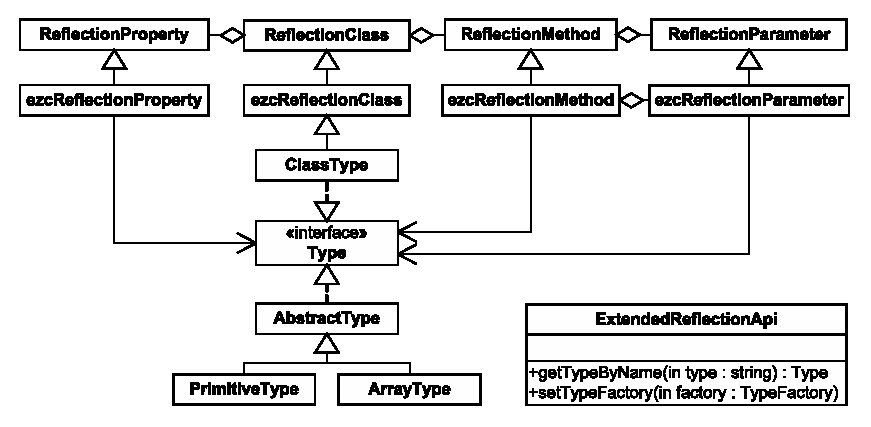
\includegraphics[width=1.00\textwidth]{figures/ezcReflection.eps}
	\caption{Class diagram of the Reflection component and its type system}
	\label{fig:ezcReflection}
\end{figure}


In Figure \ref{fig:ezcReflection} the Reflection component is shown.
For all classes of the Reflection API
new subclasses are introduced,
which provide new implementations
of the inherited methods and
additional methods to access
annotations and data types.

\paragraph{ezcReflectionClass}
ezcReflectionClass inherits from ReflectionClass
and redefines all methods which return a PHP reflection object
to return objects from the Reflection component.
In addition to that
methods for annotation handling
are introduced e.g. 
%getTags
getAnnotations,
%isTagged
hasAnnotation etc.
The generic getDocComment method is superseded
by getShortDescription and getLongDescription.
These methods return only the relevant parts
of interest from a PHPDoc comment.

%\begin{verbatim}
%class ExtReflectionClass extends ReflectionClass {
%    public void __construct(string $name)
%    public ExtReflectionMethod getMethod(string $name)
%    public ExtReflectionMethod getConstructor()
%    public ExtReflectionMethod[] getMethods()
%    public ClassType getParentClass()
%    public ExtReflectionProperty getProperty(string $name)
%    public ExtReflectionProperty[] getProperties()
%    public boolean isWebService()
%    public string getShortDescription()
%    public string getLongDescription()
%    public boolean isTagged(string $with)
%    public PHPDocTag[] getTags(string $name)
%    public ExtReflectionExtension getExtension()
%}
%\end{verbatim}

The enhancements to the Reflection API
in the classes
\textbf{ezcReflectionFunction},
\textbf{ezcReflectionMethod},
\textbf{ezcReflectionParameter},
\textbf{ezcReflectionProperty} and
\textbf{ezcReflectionExtension}
are analogue to those made in
ezcReflectionClass
and have a similar behavior.

%\begin{verbatim}
%class ExtReflectionExtension extends ReflectionExtension {
%    public void __construct(string $name)
%    public ExtReflectionFunction[] getFunctions()
%    public ExtReflectionClass[] getClasses()
%}
%
%class ExtReflectionFunction extends ReflectionFunction {
%    public void __construct(string $name)
%    public ExtReflectionParameter[] getParameters()
%    public Type getReturnType()
%    public string getReturnDescription()
%    public boolean isWebmethod()
%    public string getShortDescription()
%    public string getLongDescription()
%    public boolean isTagged(string $with)
%    public PHPDocTag[] getTags(string $name)
%}
%
%class ExtReflectionMethod extends ReflectionMethod {
%    public void __construct(mixed $class, string $name)
%    public ExtReflectionParameter[] getParameters()
%    public Type getReturnType()
%    public string getReturnDescription()
%    public boolean isWebmethod()
%    public string getShortDescription()
%    public string getLongDescription()
%    public boolean isTagged(string $with)
%    public PHPDocTag[] getTags(string $name)
%    public boolean isMagic()
%    public ClassType getDeclaringClass()
%}
%
%class ExtReflectionParameter extends ReflectionParameter {
%    public void __construct(mixed $mixed, mixed $parameter)
%    public Type getType()
%    public ClassType getClass()
%    public ExtReflectionFunction getDeclaringFunction()
%    public ClassType getDeclaringClass()
%}
%
%class ExtReflectionProperty extends ReflectionProperty {
%    public void __construct(mixed $class, string $name)
%    public Type getType()
%    public ClassType getDeclaringClass()
%}
%\end{verbatim}


\paragraph{ezcReflection}
A singleton class
called ezcReflection is defined,
which  acts as a central entry point
and factory for reflection by type name.
Therefore it provides methods necessary
to generate Reflection Objects
e.g. the method getTypeByName
will return the appropriate type object
for a given data type name specified in an annotation.
For extensibility it is also possible
to set a different factory for type objects

\paragraph{ezcReflectionTypeFactory}
A type factory has to implement the interface
ezcReflectionTypeFactory
and can be used to extend the provided type system
with additional features.

\paragraph{ezcReflectionTypeFactoryImpl}
If no type factory is provided
the default implementation ezcReflectionTypeFactoryImpl is chosen
which performs proper data type mapping
for type names provided as strings.

%\begin{verbatim}
%class ezcReflection {
%    public static ezcReflection getInstance()
%    public void setTypeFactory(ezcReflectionTypeFactory $factory)
%    public Type getTypeByName(string $typeName)
%}
%\end{verbatim}

\paragraph{ezcReflectionTypeMapper}
ezcReflectionTypeMapper is a helper class
used by the default type factory,
the primitive type class
and some of the annotation classes.
It provides mappings from various type names
which may occur in documentation
to standardized type names
or XML Schema data types.

\paragraph{ezcReflectionType}
The type interface acts as a
central interface for the type system.
It is equipped with several methods
to reflect characteristics of a data type.
For convenience and usability
also methods for an XML Schema mapping
are incorporated at this point.

%\begin{verbatim}
%interface ezcReflectionType {
%    function ezcReflectionType getArrayType();
%    function ezcReflectionType getMapIndexType();
%    function ezcReflectionType getMapValueType();
%    function boolean isArray();
%    function boolean isClass();
%    function boolean isPrimitive();
%    function boolean isMap();
%    function string toString();
%    function boolean isStandardType();
%    function string getXmlName();
%    function DOMElement getXmlSchema(DOMDocument $dom);
%}
%\end{verbatim}

\paragraph{ezcReflectionAbstractType}
The abstract type is one implementation of the type interface
and serves as an abstract base class
for ezcReflectionPrimitiveType and
ezcReflectionArrayType.

\paragraph{ezcReflectionPrimitiveType}
The primitive type is a specialization 
of ezcReflectionAbstractType
and represents the primitive types
boolean, integer, float, string and resource.

\paragraph{ezcReflectionArrayType}
The array type is the second class
to extend ezcReflectionAbstractType
and it distinguishes
between simple arrays and maps.

\paragraph{ezcReflectionClassType}
This implementation of the type interface
represents a class as a type.
For this purpose it is a specialization of ezcReflectionClass
to inherit all its capabilities,
i.e. unlike ezcReflectionPrimitiveType and ezcReflectionArrayType
the ezcReflectionClassType is tightly integrated with the Reflection API.

%\begin{verbatim}
%class ClassType extends ExtReflectionClass implements Type {
%    public Type getArrayType()
%    public Type getMapIndexType()
%    public Type getMapValueType()
%    public boolean isArray()
%    public boolean isClass()
%    public boolean isPrimitive()
%    public boolean isMap()
%    public string toString()
%    public boolean isStandardType()
%    public string getXmlName(boolean $usePrefix)
%    public DOMElement getXmlSchema(DOMDocument $dom, $namespaceXSD)
%    public void __construct(string $name)
%}
%\end{verbatim}

\paragraph{ezcReflectionDocParser}
This class parses PHPDoc comments
and provides retrieved data
in form of annotation objects.

\paragraph{ezcReflectionAnnotationFactory}
This factory creates an ezcReflectionAnnotation
object for a given annotation.

\paragraph{ezcReflectionAnnotation}
This is a generic class to represent an annotation
and it also serves as a base class for several
specialized annotation classes, e.g.
\textbf{ezcReflectionAnnotationParam},
\textbf{ezcReflectionAnnotationReturn} and
\textbf{ezcReflectionAnnotationVar}.

%\textbf{ezcReflectionAnnotationRestIn}
%\textbf{ezcReflectionAnnotationRestMethod}
%\textbf{ezcReflectionAnnotationRestOut}
%\textbf{ezcReflectionAnnotationWebMethod}
%\textbf{ezcReflectionAnnotationWebService}



%\subsubsection{Guidelines}
%----------

%\subsubsection{Algorithms}
%----------

%\subsubsection{Data structures}
%---------------

%Diagrams
%========



\section{CodeAnalyzer}\label{sec:CodeAnalyzer}
%eZ component: CodeAnalyzer, Requirements
%~~~~~~~~~~~~~~~~~~~~~~~~~~~~~~~~~
%
\subsection{Introduction}
%============
The Reflection component provides structural details about
language elements like classes and functions at runtime.
But to be able to use it, those language elements have to be loaded.
Due to the fact that most applications tend to put each class
and function definition in a separate file, it is required to load those files.

\subsubsection{Description}
%-----------
The CodeAnalyzer component is able to load entire class trees
or function libraries
%into a sandbox environment
and to examine the language elements in them.
In addition to that it is a high level interface to
perform statistical analyses and software metrics with
the Reflection package.

\subsubsection{Current implementation}
%----------------------
The current implementation can be considered as stable
and it meets all requirements which arised during
development of several tools using it.

\subsection{Requirements}\label{subsec:CodeAnalyzerRequirements}
%============
The component should be able to load entire source trees
and collect information about files respectively classes found.
Some basic software metrics should be implemented.
The required metrics include
counting the lines of code (LoC) and the number of
classes, methods, attributes, subclasses and functions.
Furthermore it should collect statistics
about the usage of documentation tags
and warn if important tags are missing.
A possible extension point would be to include abilities
to scan for coding standard violations.

\subsubsection{Design goals}
%============
The component should be easy to use through a convenient high level API
and it should be aware of possible errors in the source code files, i.e.
the CodeAnalyzer should not crash because of syntax errors in a file parsed.
This is very important because if the Code Analyzer would be that instable,
it would only be useful as a standalone tool for analyzing
smaller applications. It order to become a software metrics library
which can be included in other applications -- such as Web Service tools --
it has to be reliable.


%Special considerations
%======================

\subsubsection{Format}
%======
The package should at least work with PHP5 source code.

%Diagrams
%========

\subsection{Design}\label{subsec:CodeAnalyzerDesign}
%eZ component: CodeAnalyzer, Design
%~~~~~~~~~~~~~~~~~~~~~~~~~~~~~~~~~
%
%Introduction
%============
%
%Description
%-----------

The Code Analyzer package should be based on the reflection component
as a high level API for handling language elements.
This way it leverages the internal parser of the PHP interpreter
which can be assumed to be one of the best parsers for the language.

\subsubsection{Design description}
%------------------
The requirement of being fault tolerant has a major influence
on the design of the classes.
Since the source files have to be loaded
to employ the reflection component, some kind
of a sandbox environment is needed to ensure that errors
in the input files which stop the script execution
do not affect the Code Analyzer classes in their execution.

A simple way to achieve this is to start the analysis of the files
in a separate PHP interpreter process.
Then in case of errors only this child process stops,
but the Code Analyzer is able to report or simply ignore the error
and to continue with the next file.


\paragraph{ezcCodeAnalyzerClassLoader}
This class provides methods to recursively include
all files that contain PHP code from a given directory and all its subdirectories.
Any output of the included code will be suppressed
and files are only loaded if they do not contain
any syntax errors.
This fault tolerance is achieved by creating a new child PHP process
and performing a syntax check before loading the file into the parent PHP process.

%\verb|public static void loadDir (string $path)| 
%\verb|public static void loadFile (string $file)|


\paragraph{ezcCodeAnalyzer}
Class ezcCodeAnalyzer
implements different analyses which can be started either
separately using one of the summarization methods
or all together by calling a central collector method.

\begin{figure}[htbp]
	\centering
		\includegraphics[width=1.00\textwidth]{figures/callgraph-code_analyzer.ps}
	\caption{Static call graph for class ezcCodeAnalyzer}
	\label{fig:callgraph-code_analyzer}
\end{figure}


%Method Summary 
%\begin{verbatim}
%+static void collectMethodsStats ($classes) 
%~static int countClassesSeeingMethods 
%(array<string, mixed> $classes,  &$methodCount, int $methodCount) 
%~static int countClassesSeeingProperties
%(array<string, mixed> $classes,  &$propCount, int $propCount) 
%~static int countInheritedMethods
%(array<string, mixed> $classes) 
%~static int countOverriddenMethods
%(array<string, mixed> $classes) 
%+static int countPossibleOverriddes
%(array<string, mixed> $classes) 
%+static int countSubclasses (array<string, mixed> $classes, 
%string $class) 
%+static array<string, mixed> summarizeClasses (array<string, mixed> $classes) 
%+static array<string, mixed> summarizeClassMethods (iscReflectionClassType $class, 
% &$missingMethodComments,  &$missingParamTypes, 
%integer $missingMethodComments, integer $missingParamTypes) 
%+static array<string, mixed> summarizeClassProperties
%(iscReflectionClassType $class) 
%+static array<string, mixed> summarizeClassSignature
%(iscReflectionClassType $class) 
%+static array<string, mixed> summarizeFile (string $filename) 
%+static array<string, mixed> summarizeFunctionParameters  (iscReflectionFunction $method,  &$paramFlaws, integer $paramFlaws) 
%+static array(string=>mixed) summarizeFunctions (string[] $functions) 
%static array<string, mixed> +summarizeInSandbox ( $filename, string[] $classes) 
%+static array(string=>mixed) summarizeInterfaces (string[] $interfaces) 
%+iscCodeAnalyzer __construct ([string $path = '.']) 
%~void buildInheritanceTree () 
%+void collect () 
%~void collectClassStats () 
%~void collectFunctionStats () 
%~array flatoutStatsArray (array $array, string $basekey) 
%+array getCodeSummary () 
%+array getStats () 
%~void inspectFiles (string[] $files) 
%~void parseDir (string $path,  &$statsArray, array $statsArray) 
%+void summarizeProject ()
%\end{verbatim}


\paragraph{ezcCodeAnalyzerFileDetails}
The class ezcCodeAnalyzer uses this class
which is actually an ezcBaseStruct
as data structure for some of the details of a given file.
All data retrieval operations which include
guessing the MIME type, counting the lines of code,
and retrieving the file size
are performed during object creation.

%TODO: maybe leave it out
%\begin{figure}[htbp]
%	\centering
%		\includegraphics[width=1.00\textwidth]{figures/callgraph-file_details-with-external-calls.ps}
%	\caption{Static call graph for class ezcCodeAnalyzerFileDetails}
%	\label{fig:callgraph-file_details-with-external-calls}
%\end{figure}

%\verb|iscCodeAnalyzerFileDetails| extends \verb|ezcBaseStruct|
%
%
%Variable Summary (all protected)
%
%\begin{verbatim}
%int $countClasses <#$countClasses> 
%int $countFunctions <#$countFunctions> 
%int $countInterfaces <#$countInterfaces> 
%string $fileName <#$fileName> 
%int $fileSize <#$fileSize> 
%int $linesOfCode <#$linesOfCode> 
%string $mimeType <#$mimeType>
%\end{verbatim}
%
%
%Method Summary 
%
%\verb|public iscCodeAnalyzerFileDetails __construct ([string $file = ''])|
%
%
%Guess the mime type using the file extension 
% 
%\verb|protected boolean guessMimeType (string $file)|
% 
% 
%Use mime type to decide wheter the lines of code are counable 
% 
%\verb|protected boolean shouldCountLines (string $mime)|


%Guidelines
%----------

\subsubsection{Algorithms}
%----------

The static call graph in figure \ref{fig:callgraph-code_analyzer}
gives an impression of the collaboration between the methods.
In some methods recursion is used for traversing hierarchical 
directory and class structures but most of the methods
are not very complex. They simply collect statistics while
leveraging the Reflection component.

\subsubsection{Data structures}
%---------------
The Class Loader needs no properties
because the code loaded is stored
in PHP's internal data structures.
The Code Analyzer uses associative arrays, Reflection objects, 
and instances of ezcCodeAnalyzerFileDetails
to store the statistical data.

%Diagrams
%========



\section{WSDL}\label{sec:WSDL}
%eZ component: WSDL, Requirements
%~~~~~~~~~~~~~~~~~~~~~~~~~~~~~~~~~
\subsection{Introduction}
%============
The Web Services Description Language (WSDL) \cite{WSDL}
is one of the most important standards
for professional Web Service applications
because it allows for automated creation
of SOAP servers and clients.
The SOAP extension of PHP5 supports this
if a WSDL file is provided.
A WSDL file is an XML document
describing the interface of a Web Service.
A service provider can offer this description
to its clients which are then able
to determine the operations provided by the service
and the messages they have to sent.
In this scenario the WSDL document
serves as a contract between server and client
and both parties have to abide by it
in order to communicate successfully.

Although it is possible
to write WSDL documents by hand
the additional time and effort
do not result in a major advantage.
Due to the fact that nearly all information
needed for a WSDL description already exists
in the source code of the class or the functions
implementing the Web Service
the complete service description
can be generated automatically.

The only new information in a WSDL file
are the binding and the service access point URL.

\subsubsection{Description}
%-----------
The WSDL component generates a WSDL document
from a given service implementation.

\subsubsection{Current implementation}
%----------------------
The generator is currently in a beta stage.
The code is stable but there are some details to be improved
and some of the features have not been tested thoroughly enough.

\subsection{Requirements}\label{subsec:WSDLRequirements}
%============
The WSDL component should be able to generate a WSDL document
from a given service implementation.
Just like the SOAP server of PHP5 it should accept
a class or a set of functions as a service implementation.
The generator should be capable of building complex type definitions
for multidimensional arrays or class structures and source code documentation should be added
automatically.

\subsubsection{Design goals}
%============

The signature of the methods for adding a class or a function should
be similar to those known from PHP's SoapServer class.
Since the generator knows all details about a service
it could provide convenience methods for creating a SOAP server.
This is particularly interesting for debugging purposes
since it speeds up the testing process for service implementations.

\subsubsection{Special considerations}
%======================
To be interoperable with other platforms
the WSDL component should conform
to the Basic Profile of the
Web Services-Interoperability Organization (WS-I) \cite{BasicProfile}.
But users should also be able to create service descriptions
which do not conform to the Basic Profile,
e.g. to integrate legacy applications
with an rpc/encoded binding.

\subsubsection{Format}
%======
Of course requiring the WS-I Basic Profile implies
that the complete WSDL 1.1 standard is to be implemented.
When the WSDL 2.0 specification \cite{WSDL20} is finished
the WSDL component could be enhanced to support this as well.

%Diagrams
%========

\subsection{Design}\label{subsec:WSDLDesign}
%eZ component: WSDL, Design
%~~~~~~~~~~~~~~~~~~~~~~~~~~~~~~~~~
%
%Introduction
%============
%
%Description
%-----------
%The WSDL component generates a WSDL document from a given service implementation.
The WSDL generator utilizes the Reflection component
and the Document Object Model (DOM)
to create service descriptions in a very structured way.



\subsubsection{Design description}
%------------------

\paragraph{ezcWsdlGenerator}
This class implements the algorithms for WSDL generation.
The class diagram in figure \ref{fig:ezcWsdlGenerator.class-diagram}
shows all public methods which can be used 
to configure the generation process and
obtain the resulting WSDL document in various formats.

\begin{figure}[htbp]
	\centering
		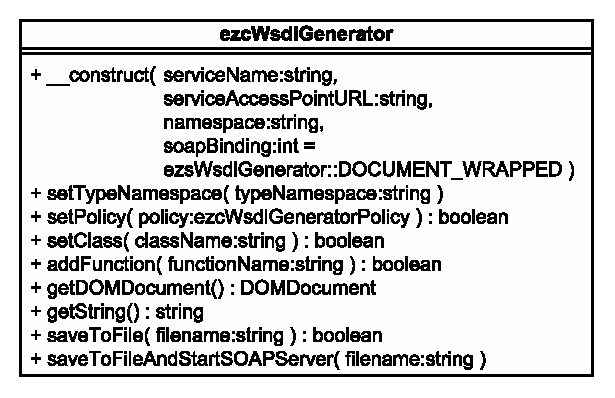
\includegraphics[width=0.70\textwidth]{figures/ezcWsdlGenerator.class-diagram.eps}
	\caption{Class diagram of ezcWsdlGenerator}
	\label{fig:ezcWsdlGenerator.class-diagram}
\end{figure}

\paragraph{ezcWsdlGeneratorPolicy}
As stated in \ref{subsec:WSDLRequirements}
the WSDL generator should
use Web Service annotations
to determine which functions to publish
in the service description.
Furthermore it should be capable of
copying the documentation for operations
from the source code to the WSDL document.
But the software projects using the generator
may have different opinions about
which methods should be selected for publication
and how much documentation should be incorporated.
Hence the generator is extensible in a way
that users can provide own implementations of the
interface ezcWsdlGeneratorPolicy.

\paragraph{ezcWsdlGeneratorDefaultPolicy}
The default implementation of the policy interface
is used if no user defined implementation is provided.
It uses the annotation \verb|@webmethod|
to identify methods for publication and
provides the short description from the PHPDoc comment
of each method as documentation for
the corresponding WSDL operation.


%\subsubsection{Guidelines}
%----------
%It must not be possible to combine
%the methods setClass and addFunction
%of ezcWsdlGenerator because
%this 


\subsubsection{Algorithms}
%----------
Through the utilization of the Reflection component
and the DOM API the methods of the WSDL generator
only have to perform the mapping between
language constructs and XML elements.

\begin{figure}[htbp]
	\centering
		\includegraphics[width=1.00\textwidth]{figures/callgraph-Generators-class.WSDLGenerator.ps}
	\caption{Static call graph of class ezcWsdlGenerator}
	\label{fig:callgraph-Generators-class.WSDLGenerator}
\end{figure}

As shown in the method call graph
in figure \ref{fig:callgraph-Generators-class.WSDLGenerator}
each WSDL element type, e.g. Operation, PortType or Binding,
is generated by a separate method in order to reduce complexity.
At some points recursion is applied
for traversing class and array structures.


\subsubsection{Data structures}
%---------------
In order to avoid redundancy in the types section of a WSDL document
the generator uses arrays for memorizing types already found.
Besides that it handles
PHP language elements with the help of reflection objects
and XML elements as DOM nodes and DOM attributes.


\subsubsection{Testing}
Since input and output may have a complex structure
testing a WSDL generator can be a challenging task.
WSDL is an interface description language
and thus a feasible method to test the generated descriptions
is to start a SOAP server with them
and verify if it behaves in the same manner as the input class.
This implies that the SOAP server has to work correctly
and that is ensured through the test cases of the SOAP extension.
These test cases probe the entire Web Service functionality
based on manually written WSDL files and also implement the
Web Services interoperability tests of the SOAP Builders community.
Therefore they can be leveraged to test the WSDL generator
through replacing the WSDL documents of the test cases
with generated versions
and comparing if the results are the same.

The test cases of the SOAP extension use PHP's test framework
which unfortunately is a conflict with the guidelines of eZ Components
stipulating PHPUnit test cases.
Thus it has to be discussed
if this exception can be tolerated for the WSDL component
or if it is technically feasible to generate unit tests
from those phpt files.


%Diagrams
%========



\section{SOAP}\label{sec:SOAP}
%eZ component: SOAP, Requirements
%~~~~~~~~~~~~~~~~~~~~~~~~~~~~~~~~~
%
\subsection{Introduction}
%============
With PHP5's SOAP extension and the WSDL component
the core standards for creating Web Services
are available to PHP developers.
But real world SOA applications need much more than that.
They have to deal with aspects
like e.g. security, synchronization or sessioning.
Therefore a large number additional Web Service standards
-- also called WS-* standards --
have evolved which commonly add new elements
to the headers of SOAP messages.
In order to be able to work with those header elements
the SOAP standard describes intermediary nodes,
which can be introduced to a communication channel
between sender and receiver.
Those SOAP Intermediaries
can add new header elements, work with them
and also remove them at a later time.
This way new communication features can be applied
transparently for sender and receiver.


\subsubsection{Description}
%-----------
The SOAP component provides enhanced versions of
the classes SoapServer and SoapClient
which are easier to use and have additional
communication features.
Furthermore it serves as a platform for implementing
WS-* standards in order to use them with PHP.
As a first standard based on that platform
this component provides a WS-Security implementation
using the Username Token Profile.


\subsubsection{Current implementation}
%----------------------
Recently the SoapServer has been redesigned
and not yet reimplemented.
But the changes are merely refactoring
in order to make the API more comprehensible.
WS-Security and the Username Token Profile
are implemented conform to the specifications.
When developing the WS-Security client a
problem occurred with PHP's SOAP extension
lacking some features.
However the current version of the SoapClient only supports the
Username Token Profile and is not as extensible
as requested in the requirements. 


\subsection{Requirements}\label{subsec:SOAPRequirements}
%============
The SOAP component should be
a platform to implement WS-* standards
as SOAP Intermediaries in client and server.
As a first standard WS-Security should be implemented
with the Username Token Profile as a first token profile.

Another problem the component should solve
is that the SOAP extension of PHP is very generic.
That is of course an advantage because it allows
to use all kinds of SOAP bindings namely
rpc/encoded, rpc/literal and document/literal.
However especially a document/literal style
is somewhat difficult to use because most
Web Service platforms prefer the special
document/wrapped flavor and in that case
the PHP application has to do wrapping and
unwrapping of return values and arguments.
But if an existing class should additionally
become accessible as a Web Service
it not acceptable to change the signatures
of the methods and the wrapping and unwrapping
should be encapsulated inside the SOAP component.

In order to facilitate the creation
of large numbers of Web Services
the SOAP component should provide
a more generic server
which can be configured with simple
deployment descriptors to handle
SOAP requests for multiple services.

Interesting features for future versions would be
to implement SOAP with Attachments \cite{SwA},
other token profiles for WS-Security and of course
other WS-* standards.


\subsubsection{Design goals}
%============
A common pattern for the realization of
SOAP Intermediaries is a handler chain.
The SOAP component should therefore
enhance client and server
with a handler chain mechanism.


\subsubsection{Special considerations}
%======================
In order to be interoperable with other platforms
the SOAP component should also conform
to the Basic Profile of the
Web Services Interoperability Organization (WS-I) \cite{BasicProfile}.


\subsubsection{Format}
%======
The security mechanisms must adhere
to the Web Services Security 1.1 \cite{WSS}
and Username Token Profile 1.1 \cite{UTP}
specifications.
Besides all enhancements the component
still has to be compliant with
the SOAP specification version 1.2 \cite{SOAP}.

%Diagrams
%========

\subsection{Design}\label{subsec:SOAPDesign}
%eZ component: SOAP, Design
%~~~~~~~~~~~~~~~~~~~~~~~~~~~~~~~~~
%
%Introduction
%============
%
%Description
%-----------
The SOAP component is based on PHP5's SOAP extension
and enhances its features by extending the classes
SoapServer and SoapClient.

\subsubsection{Design description}
%------------------

\paragraph{ezcSoapServer}
The ezcSoapServer extends the SoapServer class
with a handler chain mechanism implemented using the strategy design pattern.
Additional handlers are implemented
by extending the abstract class \textbf{ezcSoapIntermediary}
and can be added to the server
by passing an instance to the method addSoapIntermediary.
As depicted in figure \ref{fig:ezcSoapServer.class-diagram}
an ezcSoapIntermediary is actually
an extended XML parser based on the SAX API.

\begin{figure}[htbp]
	\centering
		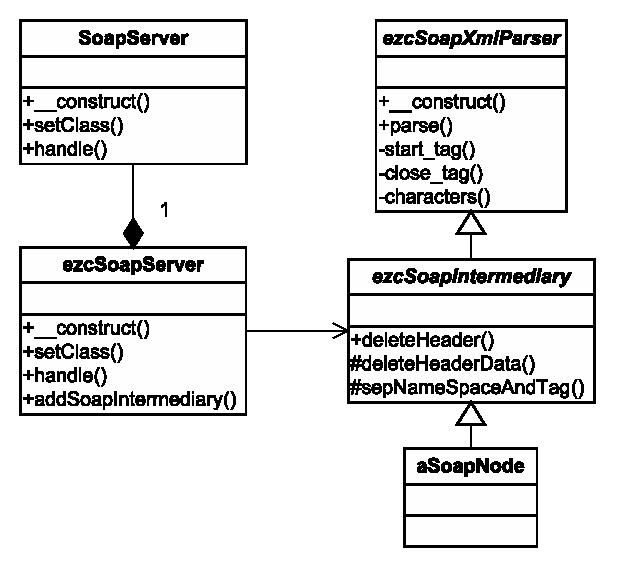
\includegraphics[width=0.60\textwidth]{figures/ezcSoapServer.class-diagram.eps}
	\caption{Class diagram of the handler chain mechanism in the SOAP server.}
	\label{fig:ezcSoapServer.class-diagram}
\end{figure}

\paragraph{ezcSoapSecurityIntermediary}
In order to implement WS-Security
this class provides a generic handler
for security headers.
The actual authentication is done
by an implementation of the interface
\textbf{ezcSoapTokenProfile}
which can be specified 
through the method setTokenProfile.

\begin{figure}[htbp]
	\centering
		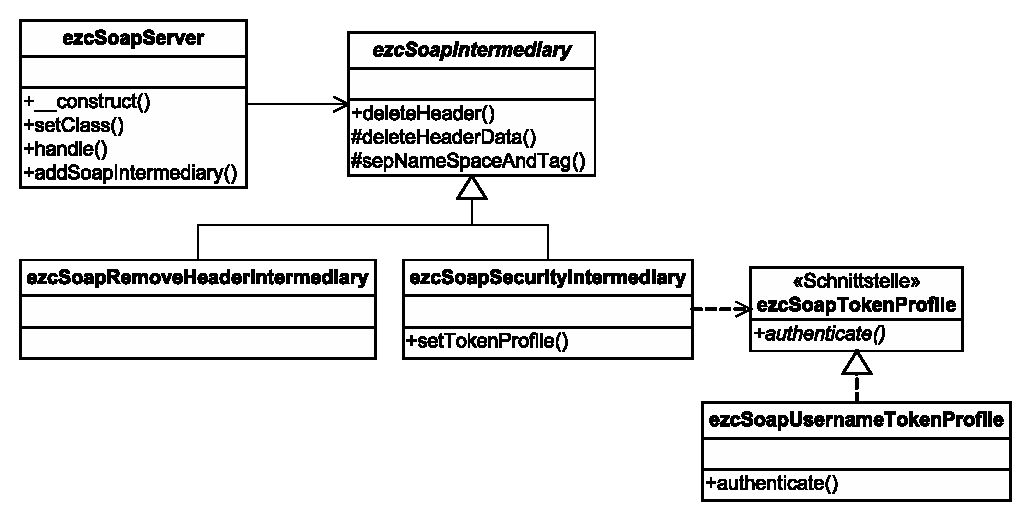
\includegraphics[width=1.00\textwidth]{figures/ezcSoapServer-with-WS-Security.class-diagram.eps}
	\caption{Class diagram of the WS-Security implementation.}
	\label{fig:ezcSoapServer-with-WS-Security.class-diagram}
\end{figure}

\paragraph{ezcSoapUsernameTokenProfile}
This class implements the authentication mechanism
specified by the Username Token Profile
of the WS-Security standard.

\paragraph{ezcSoapServerDispatcher}
To avoid writing several very similar server scripts
when providing multiple Web Services
this class provides a generic SOAP server which
can be configured via simple deployment descriptors.
It works somewhat like a front controller for SOAP
since it forwards incoming SOAP Requests
to a correspondent SOAP server instance.

\paragraph{ezcSoapDdGenerator}
This generator class provides an API
to create deployment descriptors for
ezcSoapServerDispatcher which are
actually include files returning
a PHP array with configuration settings.

\paragraph{ezcSoapAdapterGenerator}
An important requirement is
to avoid changes to the method signatures
of existing application classes
when generating document/wrapped Web Services.
This code generator builds adapter classes
which perform the unwrapping of arguments
and wrapping of return values.

\paragraph{ezcSoapClient}
Class ezcSoapClient inherits from SoapClient
and extends it with WS-Security support.
In particular the constructor method
has two new parameters for providing username and password
to the Username Token Profile authentication.
Plans for future versions are to
also apply a handler chain on the client side.
But it has not yet been examined
if that is technically feasible.
%TODO:diagram
\begin{figure}[htbp]
	\centering
		\includegraphics[width=1.00\textwidth]{figures/callgraph-SoapClient-class.SecureClient-with-external-calls.ps}
	\caption{Static call graph with external calls for class ezcSoapClient}
	\label{fig:callgraph-SoapClient-class.SecureClient-with-external-calls}
\end{figure}


\paragraph{ezcSoapClientSecurityStruct}
This data structure
contains an ezcSoapUsernameToken
and is used by ezcSoapClient
to create the SOAP headers for WS-Security.

\paragraph{ezcSoapUsernameToken}
A Username Token is a data structure
consisting of a user name,
a nonce\footnote{In cryptography this is an abbreviation for a number used once.},
a time stamp
and the encrypted password of the user.
The token is sent as a WS-Security header
from a SOAP client to a SOAP server
in order to perform authentication.

%\subsubsection{Guidelines}
%----------

\subsubsection{Algorithms}
%----------
As described in the specification
the Username Token Profile related
classes use the MD5, SHA1 and base64 algorithms.


%\subsubsection{Data structures}
%---------------

%Diagrams
%========



\section{ReST}\label{sec:ReST}
%eZ component: ReST, Requirements
%~~~~~~~~~~~~~~~~~~~~~~~~~~~~~~~~~
%
\subsection{Introduction}
%============
Representational State Transfer (ReST) is an architectural style
which can be applied to the HTTP protocol \cite{HTTP}
in order to form an alternative technology
for interoperable Web Services.
The major advantage of this concept is
that all so called ReSTful Web Services have
the same uniform and minimal interface
consisting of the HTTP methods
GET, POST, PUT and DELETE.
This improves interoperability
and interchangeability of services and 
is in contrast to SOAP where generally every service
has its own interface.
A second advantage is that all the well known standards, concepts and tools
which exist for HTTP can be reused for ReSTful Web Services.
This greatly reduces the complexity of the tool chain
and makes the services usable from virtually
every platform capable of accessing the internet.


\subsubsection{Description}
%-----------
The ReST component provides a server for
ReSTful Web Services which maps URLs
to methods of a class and handles
deserialization of incoming arguments
as well as serialization of return values.


\subsubsection{Current implementation}
%----------------------
The current implementation of the component
can be considered as stable and is
well documented by an additional paper \cite{ReSTpaper}.

\subsection{Requirements}\label{subsec:ReSTRequirements}
%============
The server of the ReST component 
should be easily configurable to serve multiple services.
It should support authentication through
the Basic or Digest authentication mechanisms of HTTP
and encapsulate XML serialization and deserialization
for PHP datatypes.

\subsubsection{Design goals}
%============
The ReST server should be generic server for all services
which is configurable through deployment descriptors
in order to minimize the effort needed to add
new services in an evolving application.

\subsubsection{Special considerations}
%======================
The component should try to ensure that the
semantics of the HTTP methods
are not violated.

\subsubsection{Format}
%======
The provided services must conform to the
HTTP 1.1 specification and the ReST concept
as described by Roy Thomas Fielding \cite{ReSTpaper},
The payloads should always be valid XML documents \cite{XML}.

%Diagrams
%========

\subsection{Design}\label{subsec:ReSTDesign}
%eZ component: ReST, Design
%~~~~~~~~~~~~~~~~~~~~~~~~~~~~~~~~~
%
%Introduction
%============
%
%Description
%-----------

\subsubsection{Design description}
%------------------
\paragraph{ezcRestServer}
This class provides a server for ReSTful Web Services.
It deserializes incoming requests into PHP data types
and calls the corespondent method of an application class.
The output of the method is serialized
and returned to the client with the HTTP response.
Additionally it is able to authenticate users
via HTTP Digest authentication.

%TODO: \paragraph{ezcRestDigestAuth}

\paragraph{ezcRestSerializer}
This interface has to be implemented by serializers
and deserializers in order to be used with the
ReST server.

\paragraph{ezcRestXmlSerializer}
This class implements a serializer
to produce XML output for a ReST service.

\paragraph{ezcRestXmlDeserializer}
The counterpart of the XML serializer is this
deserializer which is able to parse XML input.

%TODO: other resp. correct serializer classes
%TODO: \paragraph{ezcRestPearSerializer}
%TODO: \paragraph{ezcRestXbelParser}
%TODO: \paragraph{ezcRestXbelSerializer}
%TODO: \paragraph{ezcRestMapping}
%TODO: \paragraph{ezcRestMappingTable}

\paragraph{ezcRestDdGenerator}
This generator class provides an API
to create deployment descriptors for
ezcSoapServerDispatcher which are
actually include files returning
a PHP array with configuration settings.

%\subsubsection{Guidelines}
%----------

%\subsubsection{Algorithms}
%----------

%\subsubsection{Data structures}
%---------------

%Diagrams
%========



\section{WebService}\label{sec:WebService}
%eZ component: WebService, Requirements
%~~~~~~~~~~~~~~~~~~~~~~~~~~~~~~~~~
%
\subsection{Introduction}
%============

The Web Service space is nowadays split
into SOAP-based and ReSTful Web Services.
Since eZ Components incorporated solutions
for both approaches
there is a unique chance to provide a new layer of abstraction
on top of them.

\subsubsection{Description}
%-----------
The ezcWebService integrates all Web Service related
components namely ezcRest, ezcSoap and ezcWsdl and some helpers
like ezcReflection and ezcCodeAnalyzer into one powerful component.

\subsubsection{Current implementation}
%----------------------
The component is currently in a beta stage
and is used as a central tool library
for the web front-end provided by the InstantSVC project.

\subsection{Requirements}\label{subsec:WebServiceRequirements}
%============
The component should be able to
inspect an application's class tree
and generate a complete SOAP and/or ReST Web Services environment
including all classes annotated with special Web Service annotations
and/or classes specified explicitly via API calls.

\subsubsection{Design goals}
%============
The generator has to be usable by
command line interfaces as well as web front-ends
and it should be ready to be integrated
in larger SOA applications or frameworks.


\subsubsection{Special considerations}
%======================
If SOAP services are set up,
WSDL files and required adapter classes are to be generated.

\subsubsection{Format}
%======
To annotate classes for publication as Web Services
the \verb|@webservice| annotation can be set.
Methods are annotated in the style of Java
with \verb|@webmethod| for SOAP services
and using \verb|@restmethod| for ReSTful Web Services.
Classes whose instances are to be transfered
through Web Services can be annotated as \verb|@webserializable|.

%Diagrams
%========

\subsection{Design}\label{subsec:WebServiceDesign}
%eZ component: WebService, Design
%~~~~~~~~~~~~~~~~~~~~~~~~~~~~~~~~~
%
%Introduction
%============
%
%Description
%-----------

\begin{figure}[htbp]
	\centering
		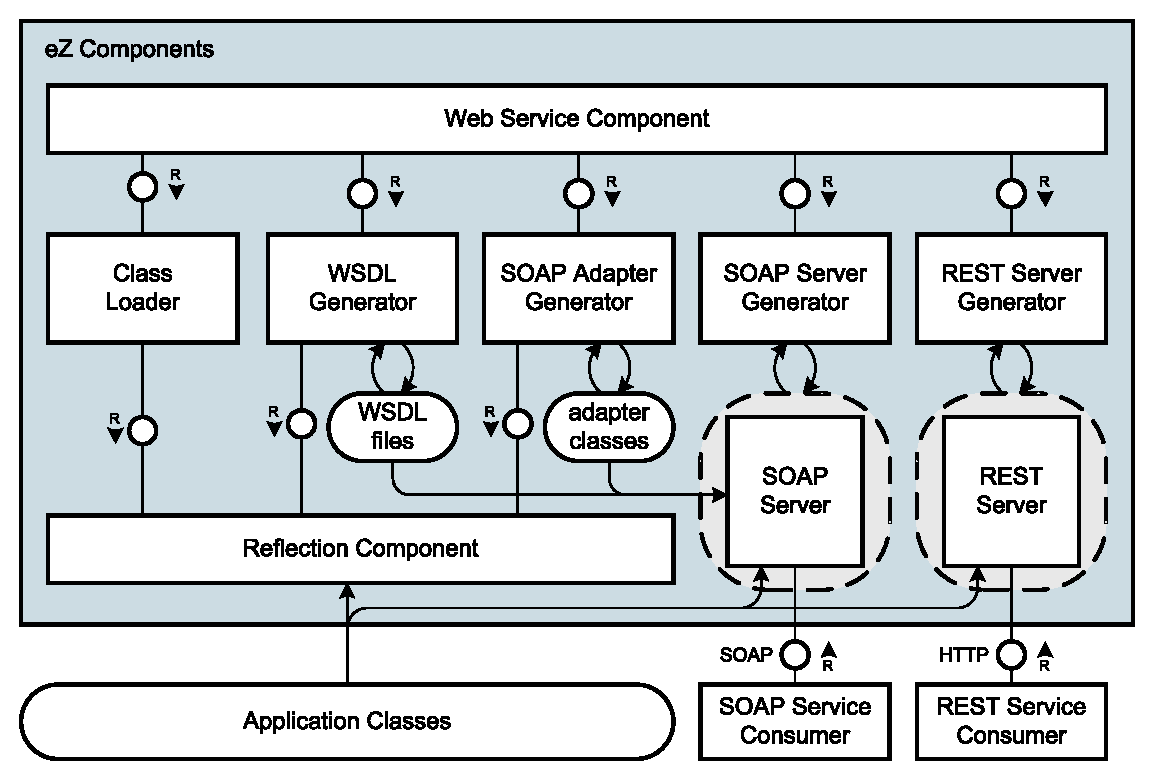
\includegraphics[width=1.00\textwidth]{figures/ezcWebService.block-diagram.eps}
	\caption{FMC block diagram of the Web Service component}
	\label{fig:ezcWebService.block-diagram}
\end{figure}
%TODO: describe model

\subsubsection{Design description}
%------------------

\paragraph{ezcWebServiceGenerator}
The Web Service component consists of a single generator class
which leverages several tools of the other components namely
ezcCodeAnalyzer, ezcReflectionClass, ezcWsdlGenerator, ezcSoapDdGenerator,
ezcSoapAdapterGenerator and ezcRestDdGenerator.


%\subsubsection{Guidelines}
%----------

\subsubsection{Algorithms}
%----------
The generator contains no complex algorithms.
It just provides a unified API
for all Web Service related components.

%\subsubsection{Data structures}
%---------------

%Diagrams
%========



\section{Conclusion}
The extension of PHP's reflection API allowed a very elegant 
implementation of a professional WSDL generator. The major advantage of 
this approach is that the algorithms for retrieving type information are 
not tied into the WSDL generator. Instead the new Reflection component is a 
reusable building block which already became a foundation for a whole 
family of Web Service helpers. But its features may be of interest for many
other PHP projects as well. The annotation mechanism could be a basis 
for using new dynamic programming techniques like e.g. aspect-oriented 
programming with PHP. 

The WSDL generator implements the complete WSDL 1.1 standard and 
supports all types of bindings. It conforms to the WS-I Basic Profile 
which guarantees interoperability with Web Service tools of other 
platforms. 

In order to select classes and methods for publication as Web Services 
annotations can be used similar to Java EE or .NET. Semantical details 
taken from the source code documentation can be introduced to generated
WSDL files.

For document/wrapped Web Services adapter classes which handle the 
wrapping and unwrapping can be generated. 

Besides WSDL there is a large number of other Web Service standards concerning 
different aspects like e.g. security, synchronization and session management. 
Those standards have in common that they add elements to the SOAP 
header. Therefore, the SOAP component introduces a handler chain 
mechanism allowing for injection of SOAP intermediaries to the 
communication channel. This way WS-* standards can be used with PHP. A 
first standard implemented on top of this platform is WS-Security with 
the Username Token Profile as a first profile providing secure 
authentication for Web Services. 

As an alternative to Web Services with complex SOAP stacks and the 
resulting time and effort ReSTful Web Services are gaining popularity 
especially among developers. On the one hand they are easy to learn and 
do not require large tool chains. On the other hand the architectural 
concept provides enhanced interoperability. As a reaction to those 
technological developments a ReST server has been designed which is able 
to host multiple services and perform authentication.

The Web Service component integrates all proposed components into one convenience 
library which allows automatic generation of SOAP and ReST servers from 
existing PHP applications. On top of that professional SOA developers 
can dynamically adapt their service landscapes to the constantly 
changing requirements. 

Since eZ Components is designed for enterprise PHP application development
it should undoubtedly incorporate professional Web Service components.

The InstantSVC project will continue to maintain a web front-end for the 
Web Service component and some command line tools for the Code Analyzer. 


\begin{thebibliography}{1}

\bibitem{SOAP}
\emph{SOAP Version 1.2 specification}, W3C Recommendation \hskip 1em plus
  0.5em minus 0.4em\relax World Wide Web Consortium (W3C), June 24, 2003.
  \newline http://www.w3.org/TR/soap/
  
\bibitem{WSDL}
\emph{Web Services Description Language (WSDL) 1.1}, W3C Note \hskip 1em plus
  0.5em minus 0.4em\relax World Wide Web Consortium (W3C), March 15, 2001.
  \newline http://www.w3.org/TR/wsdl

\bibitem{UDDI}
\emph{UDDI Version 3.0.2}, W3C Note \hskip 1em plus
  0.5em minus 0.4em\relax UDDI Spec Technical Committee Draft, OASIS, October 19, 2004.
  \newline http://uddi.org/pubs/uddi\_v3.htm
  
\bibitem{HTTP}
\emph{HTTP/1.1 specification} \hskip 1em plus
  0.5em minus 0.4em\relax RFC 2616, June 1999.
  \newline http://tools.ietf.org/html/rfc2616

\bibitem{XMLSchema}
\emph{XML Schema 1.1} \hskip 1em plus
  0.5em minus 0.4em\relax World Wide Web Consortium (W3C).
  \newline http://www.w3.org/XML/Schema

\bibitem{WSDL20}
\emph{Web Services Description Language (WSDL) 2.0}, W3C Candidate Recommendation \hskip 1em plus
  0.5em minus 0.4em\relax World Wide Web Consortium (W3C), March 26, 2006.
  \newline http://www.w3.org/TR/wsdl20

\bibitem{BasicProfile}
\emph{Basic Profile Version 1.2} \hskip 1em plus
  0.5em minus 0.4em\relax Web Services-Interoperability Organization (WS-I), Oktober 3, 2006.
  \newline http://www.ws-i.org/Profiles/BasicProfile-1.2.html
  
\bibitem{phpDocumentor}
\emph{phpDocumentor: The complete documentation solution for PHP}
  \newline http://phpdoc.org

\bibitem{PHP5Reflection}
\emph{PHP Manual: Reflection}
  \newline http://www.php.net/manual/en/language.oop5.reflection.php

\bibitem{SwA}
\emph{SOAP Messages with Attachments} \hskip 1em plus
  0.5em minus 0.4em\relax World Wide Web Consortium (W3C), December 11, 2000.
  \newline http://www.w3.org/TR/SOAP-attachments

\bibitem{WSS}
\emph{Web Services Security: 4 SOAP Message Security 1.1} \hskip 1em plus
  0.5em minus 0.4em\relax OASIS Standard Specification, February 1, 2006.
  \newline http://www.oasis-open.org/committees/download.php/16790/wss-v1.1-spec-os-SOAPMessageSecurity.pdf
  
\bibitem{UTP}
\emph{Web Services Security UsernameToken Profile 1.1} \hskip 1em plus
  0.5em minus 0.4em\relax OASIS Standard Specification, February 1, 2006.
  \newline http://www.oasis-open.org/committees/download.php/16782/wss-v1.1-spec-os-UsernameTokenProfile.pdf

\bibitem{ReSTpaper}
Fielding, Roy Thomas. \emph{Architectural Styles and the Design of Network-based Software Architectures.} \hskip 1em plus
  0.5em minus 0.4em\relax Doctoral dissertation, University of California, Irvine, 2000.
  \newline http://www.ics.uci.edu/~fielding/pubs/dissertation/top.htm

\bibitem{XML}
\emph{Extensible Markup Language (XML) 1.1 (Second Edition)}, W3C Recommendation \hskip 1em plus
  0.5em minus 0.4em\relax World Wide Web Consortium (W3C), September 29, 2006.
  \newline http://www.w3.org/TR/xml11/
  
\end{thebibliography}

\end{document}
